%#!pdfpLaTeX
%
% 古居研究室用卒業論文・特別論文のTeXテンプレートファイル
% 本ファイルは非公式である.
%
% 2022年11月17日 古居彬作成
% 2024年 9月 7日 古居彬更新
%

%%%%%%%%%%%%%%%%%%%%%%%%%%% 論文情報 %%%%%%%%%%%%%%%%%%%%%%%%%%%
%%%%% テンプレート選択 %%%%%
% \documentclass[bachelor,12pt]{infhu} % 卒論 日本語用
% \documentclass[bachelor,english,12pt]{infhu} % 卒論 英語用
% \documentclass[master,12pt]{infhu} % 修論 日本語用
\documentclass[master,english,12pt]{infhu} % 修論 英語用

%%%%% パッケージのインポート(必要に応じて追加する) %%%%%
\usepackage{amsmath, amssymb}
\usepackage[dvipdfmx]{color}
\usepackage[dvipdfmx]{graphicx}
\usepackage{tabularx}
\usepackage{booktabs}
\usepackage{multirow}
\usepackage{cite}
\usepackage{caption}
\usepackage{algorithm}
\usepackage{algpseudocode}
\captionsetup[figure]{width=\textwidth}
% \usepackage{caption}
\captionsetup[figure]{labelsep=space}
\captionsetup[table]{labelsep=space}

\title{Adaptive PolyDice Loss with Uncertainty-Based \\ Difficulty Estimation for Medical Image Segmentation} % 途中で改行する場合は\\で区切る
%¥titlewidth{} % タイトル幅 (指定するときは単位つきで)


%%%%% 著者 %%%%%
\author{Tomoya Hiroike}
\eauthor{Tomoya Hiroike} % Copyright表示で使われる

%%%% 学籍番号 %%%%
\studentid{M243422}

%%%%% 指導教員名 %%%%%
\supervisor{Assoc.\ Prof. Akira Furui} % 1つ引数をとる (役職まで含めて書く)
%\supervisor{指導教員名 役職 \and 指導教員名 役職}% 複数教員の場合,¥and でつなげる

%%%%% 提出年月 %%%%%
% \date{令和X年X月X日} % 和暦表示
\handin{2026}{2}{3} % 西暦表示

\begin{document}
\maketitle % タイトル生成
\setlength{\baselineskip}{20pt} % 行間を設定

%%%%% 目次 %%%%%
{\makeatletter
\let\ps@jpl@in\ps@empty
\makeatother
\pagestyle{empty}
\tableofcontents
}

%%%%%%%%%%%%%%%%%%%%%%%%%%% 本文 %%%%%%%%%%%%%%%%%%%%%%%%%%%
\clearpage
\section{Introduction}
Medical image segmentation is an indispensable technology in diagnostic support and treatment planning,
requiring the extraction of regions corresponding to normal or abnormal tissues.
Clinical applications are advancing rapidly, particularly in the detection of colorectal polyps~\cite{ji2022video}
and organs at risk in head and neck cancer radiotherapy~\cite{maleki2020machine}.

However, medical image segmentation presents inherent challenges.
A particularly significant issue is class imbalance.
In medical images, background regions typically occupy the majority of the image,
while target lesions often occupy only a relatively small area. Under these conditions,
the Cross-Entropy Loss~\cite{long2015fully}, which is widely used in conventional classification tasks,
becomes biased toward learning the background regions, making accurate segmentation of clinically significant small lesions and ambiguous boundaries difficult.

To address this challenge, the Dice Loss~\cite{milletari2016v}, which is robust to class imbalance,
and its many extensions have been proposed, with high performance reported in CT images~\cite{zhu2019anatomynet, 9109297}
and MRI images~\cite{KATO2024107695}. However, these loss functions have the constraint of possessing a fixed shape across all images.
Medical images exhibit significant diversity due to imaging conditions and individual differences, as well as substantial variations in lesion size and shape,
differences in tissue contrast, and boundary ambiguity; consequently, the difficulty of segmentation varies greatly from image to image.
Using a fixed loss function applies the same training signal to both easy and difficult images, which may result in insufficient learning for difficult cases.
Therefore, an approach that adaptively adjusts the loss function according to the difficulty of each image is promising.
Realizing such adaptive learning requires two elements: first, a method to flexibly control the shape of the loss function to strengthen the training signal for high-difficulty images;
and second, a difficulty metric to evaluate how challenging each image is for the model during training.

In this study, we propose an adaptive learning framework that integrates these two elements.
For controlling the shape of the loss function, we employ PolyDice Loss~\cite{polydice},
which is obtained by the polynomial expansion of Dice Loss. PolyDice Loss is suitable for adaptive learning
because it allows for continuous control of the loss function's shape using image-specific parameters.
To quantify difficulty, we use uncertainty estimation via Monte Carlo (MC)Dropout~\cite{pmlr-v48-gal16}.
MC Dropout enables the efficient estimation of the model's epistemic uncertainty by enabling dropout during inference.
This uncertainty reflects the degree of the model's lack of confidence in segmenting the image and can be utilized as an indicator of segmentation difficulty.
The proposed method dynamically controls the shape parameters of the PolyDice Loss based on estimated uncertainty metrics.
It aims to achieve efficient and robust learning by assigning steeper gradients to images for which the model currently lacks confidence, while providing gentler gradients to those where the model can already produce stable predictions.

The main contributions of this study are as follows:
\begin{enumerate}
    \item \textbf{Introduction of a dynamic quantification method for image difficulty based on uncertainty:}
    We propose a method to estimate epistemic uncertainty during inference using MC Dropout and quantify it as image-level ``learning difficulty.'' 
    This enables objective evaluation of diverse segmentation difficulties in medical images based on the model's confidence.

    \item \textbf{Construction of an adaptive control framework for the loss function based on difficulty:}
    We constructed a learning framework that adaptively controls the shape parameter of the PolyDice Loss based on the quantified difficulty metric.
    The proposed method automatically adjusts the gradients of the loss function according to the difficulty that changes with the progress of learning,
    thereby simultaneously achieving a focus on learning for difficult cases and the suppression of gradient dominance by easy cases.

    \item \textbf{Demonstration of effectiveness and versatility using multiple datasets:}
    We verified the effectiveness of the proposed method through comparative experiments using medical image datasets.
    The experimental results demonstrated that the proposed method improves segmentation accuracy compared to conventional loss functions with fixed shapes.
\end{enumerate}

\clearpage
\section{Preliminaries}
\subsection{PolyDice Loss}
医用画像セグメンテーションで広く使用されるDice Lossは,クラス不均衡に頑健であるが,全画像に対して固定的な形状を持つという制約がある.
本研究では,Dice Lossを多項式展開により拡張したPolyDice Loss\cite{polydice},特にその実用的な形式であるPolyDice-1 Lossを採用する.
PolyDice-1 Lossは,単一のパラメータ$\epsilon$で損失関数の形状を制御でき,画像の難易度に応じて勾配の急峻さを調整することが可能となる.

\subsubsection{Dice Lossの定義}
画像サイズを $H \times W$とし,ピクセル位置を $(i, j)$ で表す
$\left(i \in \{1, ..., H\}, j \in \{1, ..., W\}\right)$.
セグメンテーションタスクにおいて,モデルの予測確率マップを$\hat{\mathbf{Y}} = \{\hat{y}_{i,j}\}_{i,j} \in \mathbb R ^ {H \times W}$,
その画像に対する正解マスクを$\mathbf{Y} = \{{y}_{i,j}\}_{i,j} \in \mathbb R ^ {H \times W}$とすると,Dice Lossは次式で定義される.

\begin{equation}
    \mathcal{L}_{\text{Dice}}(\hat{\mathbf{Y}}, \mathbf{Y}) = 1 - \frac{2 \sum_{i=1}^{W} \sum_{j=1}^{H} \hat{y}_{i, j} y_{i, j}}{\sum_{i=1}^{W} \sum_{j=1}^{H}(\hat{y_{i, j}} ^ 2 + y_{i, j} ^ 2)}
\end{equation}

\subsubsection{幾何学的解釈と多項式展開}

予測確率マップ$\hat{\mathbf{Y}}$と正解マスク$\mathbf{Y}$をそれぞれ長さ$HW$のベクトル$\hat{\mathbf{y}}, \mathbf{y}$
として平坦化すると,Dice Lossは以下のように分解できる.

\begin{equation}
    \mathcal{L}_{\text{Dice}} = 1 - s \cos  \theta
\end{equation}
ここで,$s = \frac{2 \langle \hat{\mathbf{y}}, {\mathbf{y}} \rangle}{\Vert \hat{\mathbf{y}} \Vert ^ 2 + \Vert {\mathbf{y}} \Vert ^ 2}$はスケール成分,
$\theta = \frac{\langle \hat{\mathbf{y}}, {\mathbf{y}}\rangle}{\Vert \hat{\mathbf{y}} \Vert \Vert {\mathbf{y}}\Vert}$は2つの
ベクトル間の角度を表す.この分解により,Dice Lossはスケール成分$s$と$\cos \theta$の積として理解できる.

方向成分$\cos \theta$に対してTaylor展開を適用することで,PolyDice Lossの多項式表現を導出する.
つまり$\theta \approx 0$(予測と正解が大きく異ならない)と仮定し,$\cos{\theta}$を$\theta = 0$まわりでテイラー展開すると以下のように近似できる.
\begin{equation}
    \cos{\theta} = 1 - \frac{\theta ^ 2}{2!} + \frac{\theta ^ 4}{4!} - \cdots
\end{equation}
これをDice Lossに代入し,整理するとPolyDiceの一般形が得られる:

\begin{equation}
    \mathcal{L}_{\text{PolyDice}} = (1 - s) + s \sum_{k = 1}^{\infty} \alpha_k \theta ^ {2k}
\end{equation}
ここで, $\alpha_k=\frac{(-1)^{k-1}}{(2k)!}$は各Taylor項の符号係数である.

\subsubsection{PolyDice-1 Loss}

実用的な観点から,\cite{leng2022polyloss}のアプローチに従い,第$1$項のみを調整可能とするPolyDice-1 Lossを採用する:
\begin{equation}
    \mathcal{L}_{\text{PolyDice-1}} = (1 - s) + s \left(\frac{1}{2} + \epsilon\right) \theta^2
\end{equation}
ここで,$\epsilon \in \mathbb{R}$は損失関数の形状を制御するハイパーパラメータである.
図\ref{polydice}に,$\epsilon$に応じたPolyDice-1 Lossの形状変化を示す.
$\epsilon > 0$では予測誤差に対するペナルティが強化され,$\epsilon < 0$では緩和される.

\clearpage

\begin{figure}
    \includegraphics[width=\columnwidth]{figure/loss.pdf}
    \caption{Plot of PolyDice-1 Loss($s = 0.1$)}
    \label{polydice}
\end{figure}

\clearpage

\subsection{MC Dropoutの原理と応用}

Dropoutは元々,ニューラルネットワークの過学習を防ぐ正則化手法として提案された\cite{JMLR:v15:srivastava14a}.
訓練時に各層のニューロンを確率$p$でランダムに不活性化することで
モデルの汎化性能を向上させる.通常,推論時にはDropoutは無効化され,全ニューロンが活性化される.

MC Dropoutは,学習時のみだけでなく,推論時にもDropoutを有効にすることで,モデルの認識的不確実性を推定する手法である.
通常,推論時の出力は決定論的であるが,Dropoutを有効にすることで,
異なるサブネットワークが形成され、確率的な出力が得られる.
同一入力に対してこの確率的な推論を複数回実行して得られる予測結果の分布は、
Bayesian Neural Networkにおける予測事後分布近似とみなせ,変分推論の一種として解釈できる.

提案法では,このMC Dropoutを学習過程の各段階で適用する.
具体的には,$\tau$エポックごとに推論フェーズを挿入し,その時点でのモデルが各セグメンテーションをどの程度「難しい」と感じているかを定量化する.



\clearpage
\section{Proposed Method}
\subsection{Overview}Let $\mathcal{D} = \{(\mathbf{X}_n, \mathbf{Y}_n)\}_{n=1}^{N}$ denote the training dataset,
where $N$ is the total number of training images, $\mathbf{X}_n \in \mathbb{R}^{H \times W \times C}$ is the $n$-th input image ($C$ is the number of channels),
and $\mathbf{Y}_n = \{y_{n,i,j}\}_{i,j} \in \mathbb{R}^{H \times W}$ is the corresponding ground truth mask.
In uncertainty estimation using MC Dropout, $T$ stochastic inferences are performed for each image.
We denote the predicted probability map in the $t$-th inference ($t \in \{1, \ldots, T\}$) as $\hat{\mathbf{Y}}_n^{(t)} = \{\hat{y}_{n,i,j}^{(t)}\}_{i,j}$.

Fig.~\ref{method} illustrates the overview of the proposed method. The design of this method is primarily based on the following two perspectives.
First, the difficulty assessment for training samples is dynamically updated during the learning process.
Since image difficulty is not absolute but relative, changing with the model's training progress,
sequentially re-evaluating difficulty based on the current state of the model allows learning to focus on images where the model currently lacks confidence.
Second, epistemic uncertainty is suitable as a quantitative metric for difficulty. Since epistemic uncertainty stems from the model's lack of knowledge,'' 
it directly reflects unlearned patterns or regions where the model is hesitant. Therefore, it allows for the appropriate quantification of how unconfident the model is,''
which can be improved through learning, without being affected by noise.

In the proposed method, MC Dropout is used every $\tau$ epochs during training to perform multiple inferences for each image,
and uncertainty is quantified from the variance of the predictions.This uncertainty information reflects the degree of the model's lack of confidence
in the segmentation of that image.Subsequently, this uncertainty information is aggregated on a per-image basis to dynamically control the shape of the PolyDice Loss,
assigning steeper gradients to difficult images and gentler gradients to easy images.By applying the updated $\epsilon$ to the training in the next $\tau$ epochs,
we realize adaptive learning that dynamically changes the optimization weighting according to the progress of learning.

\clearpage

\begin{figure}
    \includegraphics[width=\columnwidth]{figure/method.pdf}
    \caption{Overview of the proposed adaptive learning framework.The process consists of two phases: uncertainty estimation and adaptive training. Every $\tau$ epochs,
    the model evaluates image difficulty using MC Dropout and updates the loss shape parameter $\epsilon$. This dynamic control assigns steeper gradients to harder samples, enabling difficulty-aware optimization.}
    \label{method}
\end{figure}

\clearpage

\subsection{Quantification of Image Difficulty Based on Uncertainty}
\subsubsection{MC Dropout Inference During Training}
In the proposed method, the learning process is divided into two phases:
an initial training phase and an adaptive training phase.
The period from epoch $1$ to $E_0 - 1$ is defined as the initial training phase,
where training is performed with the loss shape parameter $\epsilon$ fixed at $0$.
The reason for establishing this period is that the feature representation of the model is immature in the early stages of learning,
and uncertainty at this stage depends more on the model's initialization than on the intrinsic difficulty of the image.
$E_0$ is set as the number of epochs sufficient for the model to acquire basic segmentation capabilities.
In the adaptive training phase ($e \geq E_0$), the re-evaluation of uncertainty and the update of $\epsilon$ are performed every period $\tau$.
That is, the update is executed before the start of learning for epochs satisfying $e \in \{E_0, E_0+\tau, E_0+2\tau, \ldots\}$.
During the update, the model parameters $\mathbf{W}$ at that point are fixed, and $T$ stochastic inferences are performed for each image
$\mathbf{X}_n$ in the training data with a Dropout rate $p \in (0,1)$.Let the obtained set of predictions be 
$\{\hat{\mathbf{Y}}_n ^ {(t)}\}_{t=1}^{T}$:
\begin{equation}
    \hat{\mathbf{Y}}_n ^ {(t)} = f_{\mathbf{W}}(\mathbf{X}_n; \mathbf{z}^{(t)}), \quad \mathbf{z}^{(t)} \sim \text{Bernoulli}(1-p)
\end{equation}
Here, $\mathbf{z}^{(t)}$ is the Dropout mask for the $t$-th inference, and $\hat{\mathbf{Y}}_n ^ {(t)}$ is the resulting predicted probability map.
The model's epistemic uncertainty is quantified from the variance of predictions obtained through this stochastic inference.

\subsubsection{Calculation of Pixel-wise Uncertainty Metrics}For the $T$ predicted images obtained by MC Dropout,
we calculate the Mutual Information $I_{n, i, j}$, which can directly capture epistemic uncertainty, as a pixel-wise uncertainty metric.
\begin{equation}
    I_{n, i, j} = \underbrace{H\left( \frac{1}{T} \sum_{t=1}^{T} \hat{y}_{n, i,j}^{(t)} \right)}_{\text{Entropy of Mean}} - \underbrace{\frac{1}{T} \sum_{t=1}^{T} H\left( \hat{y}_{n, i,j}^{(t)} \right)}_{\text{Mean of Entropy}}
\end{equation}
Here, $H(p)$ is the binary entropy function for binary classification, defined as follows:
\begin{equation}
    H(p) = -p \log p - (1-p) \log (1-p)
\end{equation}
Mutual Information is widely used as a metric to evaluate the uncertainty accompanying model predictions and to isolate its underlying factors.
It quantifies epistemic uncertainty by subtracting the expected entropy (the mean of the entropy of individual inferences),
which indicates aleatoric uncertainty derived from data-inherent noise and ambiguity, from the predictive entropy,
which is the uncertainty of the predictive distribution after averaging $T$ inference results (indicating uncertainty from both data and model).
High values in a region suggest that the model has not sufficiently learned that area.

\subsubsection{Aggregation to Image Level}
The mean value of the pixel-wise mutual information, after outlier removal, is quantified as the difficulty metric for the entire image.
In medical image segmentation, there is an extreme class imbalance where background regions occupy the majority of the image,
while the lesion areas of interest are extremely small. Background regions are generally easy to infer,
and their uncertainty tends to take extremely low values. Therefore, if the average uncertainty is calculated over the entire image,
the low values from the massive number of background pixels may dominate the overall difficulty metric, failing to properly quantify the local difficulty of the lesion that should be captured.
Therefore, to sensitively reflect the difficulty of lesion detection, the proposed method calculates the average mutual information restricted to the lesion region in the ground truth mask.
Let $\Omega_n$ be the entire image domain, and $\mathcal{P}_n = \{(i,j) \in \Omega \mid y_{i,j} = 1\}$ be the set of pixels in the positive region of the ground truth mask.
Here, the calculated mutual information may contain sporadic noise or extreme outliers, which can destabilize the quantification of the difficulty metric.
Therefore, prior to calculating the score, statistical outlier removal is performed. Specifically,
let $\mu_{\mathcal{P}_n}$ be the mean and $\sigma_{\mathcal{P}_n}$ be the standard deviation of the mutual information within the region $\mathcal{P}_n$.
The valid pixel set $\mathcal{P}_n'$ is defined as follows:
\begin{equation}
    \mathcal{P}_n' = \left\{ (i,j) \in \mathcal{P}_n \mid \mu_{\mathcal{P}_n} - 2\sigma_{\mathcal{P}_n} \leq I_{n, i, j} \leq \mu_{\mathcal{P}_n} + 2\sigma_{\mathcal{P}_n} \right\}
\end{equation}
The rationale for adopting $2\sigma_{\mathcal{P}_n}$ as the threshold is based on the concept of statistical confidence intervals.
Assuming the distribution of mutual information approximates a normal distribution, approximately $95\%$ of all data falls within the range of $\pm 2\sigma$ centered on the mean.
Therefore, by rejecting data outside this range, statistically singular extreme values (outliers) are effectively removed, enabling robust difficulty estimation that reflects the main features of the lesion.
Using this valid set $\mathcal{P}_n'$, the difficulty score $D_n$ for the entire image is calculated as:
\begin{equation}
    D_n = \frac{1}{|\mathcal{P}_n'|} \sum_{(i,j) \in \mathcal{P}_n'} I_{n, i,j}
\end{equation}
Here, $|\mathcal{P}_n'|$ represents the number of pixels in the positive region after outlier removal. Note that for images with no positive region, $D_n = 0$.

Next, to determine the relative difficulty of each sample, normalization is performed based on the difficulty score distribution of the entire dataset.
The purpose here is to absorb numerical scale differences between images and evaluate how relatively difficult each image is within the overall distribution.
Given the set of scores $\{D_n\}_{n = 1} ^ N$ for the entire dataset, let $D_q$ be the $q$-th percentile value and $\sigma_D$ be the standard deviation.
The normalized score is calculated as follows:
\begin{equation}
    D_{n} ^ {\text{norm}} = \frac{D_n - D_{q}}{\sigma_D + \delta}
\end{equation}
Here, $\delta > 0$ is a small constant for numerical stability.Subtraction by $D_q$ serves to center the input for the control function described later.
By using the $q$-th percentile instead of the mean of the distribution, the baseline for difficulty can be flexibly set without being affected by outliers,
even in distributions dominated by easy samples.Division by $\sigma_D$ unifies the scale,
serving to adjust the sensitivity of the control function so that it does not depend on the scale of uncertainty specific to each dataset.

\subsection{Adaptive Loss Shape Control}\
subsubsection{Design of the Control Function}
Based on the obtained difficulty metric $D_{n} ^ {\text{norm}}$, the shape parameter $\epsilon$ of the PolyDice-1 Loss is dynamically updated.
We use the following sigmoid-based control function for the update equation.
\begin{equation}
    \epsilon = \epsilon_{\text{min}} + (\epsilon_{\text{max}} - \epsilon_{\text{min}}) \sigma(k \cdot D_{n} ^ {\text{norm}})
\end{equation}
Here, $\sigma(x) = (1 + e^{-x})^{-1}$ is the standard sigmoid function, $k > 0$ is a parameter, and $\epsilon_{\text{min}}, \epsilon_{\text{max}}$ represent the variation range of $\epsilon$.
The reason for adopting the sigmoid function in this method lies in its boundedness and smoothness.Abrupt switching, such as with a step function,
ay compromise training stability,while a linear function may cause the parameter $\epsilon$ to deviate from the appropriate range $[\epsilon_{\text{min}}, \epsilon_{\text{max}}]$.
By using the sigmoid function, it is possible to smoothly transition from low to high difficulty regions while strictly constraining the output value within a predetermined range.
The parameter $k$ controls the response sensitivity of the function; as shown in Fig.~\ref{sigmoid}, a larger value results in a steeper boundary for difficulty judgment,
while a smaller value results in a smoother transition.Through this control, a large $\epsilon$ is assigned to difficult images (large $D_{n} ^ {\text{norm}}$),
making the gradient of the loss function steeper.This implies giving a larger loss value and gradient for the same prediction error,
resulting in the relative strengthening of the learning signal from difficult images.On the other hand, a small $\epsilon$ is assigned to easy images that have already been sufficiently learned,
preventing overfitting while concentrating learning resources on difficult images.The updated $\epsilon$ is applied to training, enabling the model to focus on learning difficult images.

\clearpage

\begin{figure}
    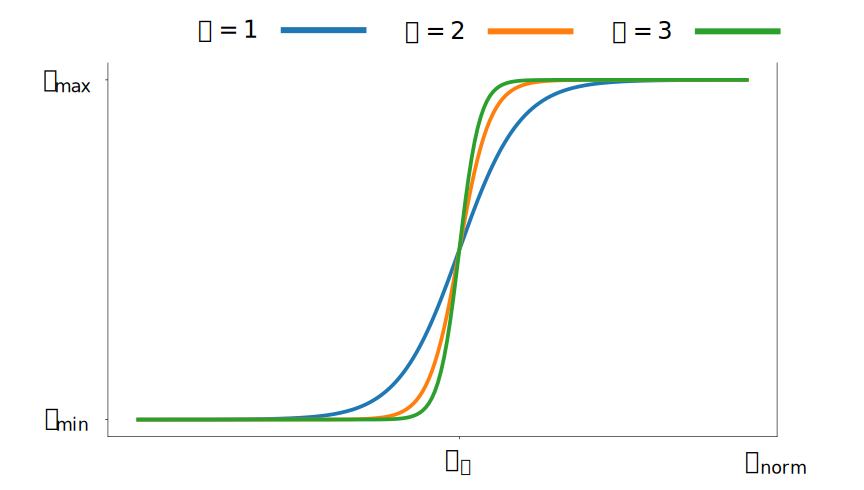
\includegraphics[width=\columnwidth]{figure/sigmoid_sensitivity.pdf}
    \caption{Sigmoid-based control function for loss shape parameter $\epsilon$}
    \label{sigmoid}
\end{figure}

\clearpage

\subsubsection{Learning Algorithm}
Algorithm \ref{alg:proposed_method} presents the detailed algorithm.The learning process consists of two components: adaptive control,
which performs difficulty evaluation and loss parameter updates, and the training phase, which actually updates the model parameters.At the start of training,
the model parameters $\mathbf{W}$ are initialized, and the loss shape parameter $\epsilon$ for all images is initialized to $0$.
In the case where $E_0 > 0$, the period from epoch $1$ to $E_0 - 1$ is the initial training phase, and training is performed with the standard PolyDice-1 Loss fixing $\epsilon=0$.Through this period,
the model acquires the fundamental feature representations necessary for uncertainty estimation.If $E_0 = 0$, adaptive control begins from the first epoch.In the adaptive training phase ($e \geq E_0$),
adaptive control is executed every $\tau$ epochs.Here, following the procedure described in Section 3.2, $\epsilon$ for each image is updated through uncertainty metric estimation via MC Dropout inference,
aggregation to image units, and normalization.Note that during the adaptive control stage, the model parameters $\mathbf{W}$ are fixed,
and only the update of the loss function shape parameter $\epsilon$ is performed.In the subsequent training phase (Epoch $e$),
mini-batch learning is performed using the updated $\epsilon$.Specifically, let $\mathcal{B} \subset \{1, \dots, N\}$ be the set of indices of images constituting a randomly sampled mini-batch.
The objective function $\mathcal{L}$ to be optimized is defined as the average of the PolyDice-1 Loss using the shape parameter $\epsilon_n$ individually assigned to each image $n \in \mathcal{B}$ in the batch, as follows:

\begin{equation}
    \mathcal{L} = \frac{1}{|\mathcal{B}|} \sum_{n \in \mathcal{B}} \mathcal{L}_{\text{PolyDice-1}}(\hat{\mathbf{Y}}_n, \mathbf{Y}_n; \epsilon_n)
\end{equation}

Here, $\mathcal{L}_{\text{PolyDice-1}}(\cdot; \epsilon_n)$ represents the loss function for a single image with parameter $\epsilon_n$ applied.
By applying a different $\epsilon_n$ to each image in the batch in this way, it becomes possible to simultaneously assign steep gradients to images determined to be high difficulty and gentle gradients to low difficulty images.
Finally, the model parameters $\mathbf{W}$ are optimized by gradient descent based on this loss function $\mathcal{L}$.
By repeating this cycle, it becomes possible to focus learning on difficult images according to the model's training progress.

\clearpage

\begin{algorithm}[t]
    \caption{Uncertainty-based Adaptive PolyDice-1 Loss Learning Algorithm}
    \label{alg:proposed_method}
    \begin{algorithmic}[1]
        \small
        \Require Training dataset $\mathcal{D} = \{(\mathbf{X}_n, \mathbf{Y}_n)\}_{n=1}^{N}$
        \Require Model $f_{\mathbf{W}}$, Max epochs $E$
        \Require \textbf{Hyperparameters:} Dropout probability $p$, Start epoch $E_0$, Interval $\tau$, MC iterations $T$, Normalization percentile $q$, Slope $k$, Range $[\epsilon_{\text{min}}, \epsilon_{\text{max}}]$
        
        \State Initialize model parameters $\mathbf{W}$
        \State Initialize loss parameters $\epsilon_n \leftarrow 0$ for all $n \in \{1, \dots, N\}$
        
        \For{$e = 1$ \textbf{to} $E$}
            \If{$e \geq E_0$ \textbf{and} $(e - E_0) \pmod \tau = 0$}
                \State Set model to evaluation mode (enable Dropout)
                
                \For{$n = 1$ \textbf{to} $N$}
                    \For{$t = 1$ \textbf{to} $T$}
                        \State $\hat{\mathbf{Y}}^{(t)} = f_{\mathbf{W}}(\mathbf{X}_n; \mathbf{z}^{(t)}), \quad \mathbf{z}^{(t)} \sim \text{Bernoulli}(1-p)$
                    \EndFor
                    
                    \State Calculate pixel-wise Mutual Information (Eq. 9):
                    \State $I_{n, i,j} = H\left( \frac{1}{T} \sum_{t=1}^{T} \hat{y}_{n, i,j}^{(t)} \right) - \frac{1}{T} \sum_{t=1}^{T} H\left( \hat{y}_{n, i,j}^{(t)} \right)$
                    
                    \If{positive region $\mathcal{P}_n \neq \emptyset$}
                        \State Compute $\mu_{\mathcal{P}_n}, \sigma_{\mathcal{P}_n}$ from $\{I_{n,i,j} \mid (i,j) \in \mathcal{P}_n\}$
                        \State Identify valid pixels: $\mathcal{P}_n' = \{(i,j) \in \mathcal{P}_n \mid |I_{n,i,j} - \mu_{\mathcal{P}_n}| \leq 2\sigma_{\mathcal{P}_n} \}$
                        \State $D_n = \frac{1}{|\mathcal{P}_n'|} \sum_{(i,j) \in \mathcal{P}_n'} I_{n, i,j}$
                    \Else
                        \State $D_n \leftarrow 0$ \Comment{Handle negative samples}
                    \EndIf
                \EndFor

                \State \textbf{Step 2: Normalization \& $\epsilon$ Update}
                \State Compute $q$-percentile $D_q$ and std $\sigma_D$ from $\{D_n\}_{n=1}^N$
                \For{$n = 1$ \textbf{to} $N$}
                    \State Normalize score (Eq. 13): $D_{n, \text{norm}} = \frac{D_n - D_{q}}{\sigma_D + \delta}$
                    \State Update $\epsilon_n$ (Eq. 14): $\epsilon_n \leftarrow \epsilon_{\text{min}} + (\epsilon_{\text{max}} - \epsilon_{\text{min}}) \sigma(k \cdot D_{n, \text{norm}})$
                \EndFor
            \Else
                \State \Comment{Keep current $\epsilon_n$ (Note: $\epsilon_n=0$ if $e < E_0$)}
            \EndIf

            \State
            \State Set model to training mode (disable MC Dropout)
            \For{each minibatch $\mathcal{B} \subset \{1, \dots, N\}$}
                \State Compute batch loss with sample-specific $\epsilon_n$ (Eq. 15):
                \State \quad $\mathcal{L} = \frac{1}{|\mathcal{B}|} \sum_{n \in \mathcal{B}} \mathcal{L}_{\text{PolyDice-1}}(\hat{\mathbf{Y}}_n, \mathbf{Y}_n; \epsilon_n)$
                \State Update parameters: $\mathbf{W} \leftarrow \mathbf{W} - \eta \nabla_{\mathbf{W}} \mathcal{L}$
            \EndFor
        \EndFor
        \State \Return Trained parameters $\mathbf{W}$
    \end{algorithmic}
\end{algorithm}

% \clearpage

\clearpage
\section{Experiments}
提案法の有効性を検証するために,医用画像データセットを用いた実験を行った.


\subsection{実験設定}
\subsubsection{データセットおよび実装の詳細}
CVC-ClinicDBデータセット\cite{BERNAL201599}データセットおよびKvasir-SEGデータセット\cite{jha2020kvasir}を用いて実験を行った.
CVC-ClinicDBデータセットは$612$枚の大腸内視鏡画像($384 \times 288$ pixel),Kvasir-SEGデータセットは$1000$枚の大腸内視鏡画像で,
いずれも大腸内視鏡画像とそれに対応するポリープの正解マスクから構成される.

セグメンテーションモデルには表\ref{tab:unet_architecture}に示される構造のU-Net\cite{ronneberger2015u}を採用した.
学習にはAdam optimizer\cite{kingma2014adam}を使用し,バッチサイズ$32$, 学習率$10 ^ {-3}$に設定した.
損失関数にはPolyDice-1 Loss($\epsilon = 0$)を用いた.
前処理として全画像を$W = 224$ pixel, $H = 224$ pixelにリサイズし,訓練時には
$50\%$の確率で上下左右反転および明度・コントラストの変更を適用した.
最大エポック数$E$は$200$に設定した.

MC Dropoutによる不確実評価は,$\tau=10$エポックごとに実施した.
Dropout層はエンコーダの最終ブロックとデコーダの最終ブロックに配置し,
各評価時には,$p = 0.5$で$N = 10$回の確率的推論を行った.
またバッチ内の難易度指標の正規化時のパーセンタイルは$p = 25$に設定し,
適応的学習の開始エポックは$E_{\text{start}} = 0$とし,
$\epsilon_{\text{min}}=0$, $\epsilon_{\text{max}}=0.5$, $k=2$とした.


\subsubsection{比較条件および比較指標}
適応的学習の有効性を評価するため,複数の条件下で比較実験を行った.
まず,医用画像セグメンテーションにおける標準的なベースラインとしてDice Lossを検討し,
併せてクラス不均衡問題に対処する代表的手法であるFocal Loss\cite{lin2017focal}とも比較を行った.
また易しいサンプルの重みを下げる割合を調整するパラメータは$\gamma=2$と設定した.
次に,PolyDice-1 Lossにおけるパラメータ $\epsilon$を動的に制御することの有効性を検証するため,
$\epsilon$ を固定値とした場合との比較を行った.
これには,Dice Lossを近似した $\epsilon=0$ の設定に加え,予備実験により探索されたデータセットごとの最適な固定値を用いたPolyDice-1 Lossが含まれる.
これらの比較手法と,不確実性指標に基づいて $\epsilon$ を適応的に更新する提案法の
セグメンテーション精度を比較することで,提案手法の有効性を検証する.

またセグメンテーションの性能の評価には,Dice係数,IoU,Precision,Recallを用いた.

\clearpage

\begin{table}[t]
    \centering
    \caption{Overview of the U-Net Architecture}
    \label{tab:unet_architecture}
    \begin{tabular}{lc}
        \toprule
        \textbf{Layer} & \textbf{Output Size} \\
        \midrule
        % ★★★ 表示するテキストを追加 ★★★
        \multicolumn{2}{c}{\textit{--- Encoder ---}} \\
        Input & $224 \times 224 \times 3$ \\
        inc (DoubleConv) & $224 \times 224 \times 64$\\
        down1 (MaxPool + DoubleConv) & $112 \times 112 \times 128$ \\
        down2 (MaxPool + DoubleConv) & $56 \times 56 \times 256$ \\
        down3 (MaxPool + DoubleConv) & $28 \times 28 \times 512$ \\
        down4 (MaxPool + DoubleConv) & $14 \times 14 \times 512$ \\
        \midrule
        % ★★★ 表示するテキストを追加 ★★★
        \multicolumn{2}{c}{\textit{--- Decoder ---}} \\
        up1 (Upsample + DoubleConv) & $28 \times 28 \times 256$ \\
        up2 (Upsample + DoubleConv) & $56 \times 56 \times 128$ \\
        up3 (Upsample + DoubleConv) & $112 \times 112 \times 64$ \\
        up4 (Upsample + DoubleConv) & $224 \times 224 \times 64$ \\
        \midrule
        outc (Conv2d) & $224 \times 224 \times 2$ \\
        \bottomrule
    \end{tabular}
\end{table}

\clearpage

\begin{table}[t]
    \centering
    \caption{Performance Comparison with Existing Loss Functions on Kvasir-SEG Dataset}
    \label{tab:results}
    \begin{tabular}{ccccc} % lcccc から ccccc に変更(全て中央揃え)
        \toprule
        Method & Dice & IoU & Precision & Recall \\ % Dice Coefficient -> Dice に短縮
        \midrule
        Dice Loss & 0.7895 & 0.7021 & 0.8281 & 0.8154 \\
        Focal Loss ($\gamma = 2$) & 0.7192 & 0.6082 & 0.8634 & 0.6769 \\
        PolyDice-1 ($\epsilon=0$) & 0.8095 & 0.7198 & 0.8461 & 0.8268 \\ % fixed, .0 を削除
        PolyDice-1 (Opt. $\epsilon$) & 0.8095 & 0.7198 & 0.8461 & 0.8268 \\ % optimized, fixed を短縮
        \midrule
        Adaptive PolyDice-1 & \textbf{0.8272} & \textbf{0.7440} & \textbf{0.8707} & \textbf{0.8397} \\
    \bottomrule
    \end{tabular}
\end{table}

\clearpage
\section{Conclusion}
本稿では,医用画像セグメンテーションにおける適応的学習手法を提案した.
提案法では,MC Dropout を用いてモデルの認識的不確実性を定量化し,これを画像の
セグメンテーション難易度の指標として活用する.
得られた難易度指標に基づき,PolyDice-1 Loss の形状パラメータを動的に制御することで,
モデルの学習状態に応じた適応的な勾配調整を実現した.この動的制御により,結果として困難な症例の学習が促進されることを確認した.

CVC-ClinicDB および Kvasir-SEG データセットを用いた評価実験において,
提案法は Dice Loss や FocalLoss などの既存手法に加え,
テストデータに対して最適化された固定パラメータ設定をも上回る性能を達成した.
特に,従来手法では抽出が困難であった症例群に対して,CVC-ClinicDB において Dice 係数が$0.32$向上するなど,提案する適応的学習
戦略が困難な病変の検出に有効であることが示された.

本手法の限界として,不確実性推定のために複数回の推論を要するため,標準的な学習と比較して計算コストが増加する点が挙げられる.
また,現在の枠組みは経験的に設定されたハイパーパラメータに依存しており,これらをデータセットに応じて自動最適化する手法の確立が課題として残されている.
今後は,計算効率の改善に取り組むとともに,CTやMRIなどの3次元医用画像へ本手法を拡張し,より広範な臨床タスクにおける有効性を検証する予定である.


\clearpage
\section*{Acknowledgement}
\addcontentsline{toc}{section}{Acknowledgement}
I would like to express my sincere gratitude to my supervisor, Associate Professor Akira Furui, for his constant and enthusiastic guidance and great encouragement throughout the course of this research.
Associate Professor Furui provided me with detailed and careful instruction on every aspect of my work, ranging from discussions on the direction of the research to thesis writing and presentation techniques.
Although I had mixed feelings of anticipation and anxiety when I was first assigned to the laboratory, thanks to his advice—at times kind and at times strict—I was able to push forward with my research without hesitation.

I would like to express my deep appreciation to Professor Hiroaki Mukaidani and Associate Professor Zu Soh, who served as my sub-supervisors,
for their valuable advice during the interim presentation. The insightful comments and sharp feedback I received from them served as extremely important guidelines for improving the quality of this research and deepening the discussion.

I am also deeply grateful to Assistant Professor Hiroaki Aizawa for providing valuable opinions from multiple perspectives during our collaborative research.
He taught me how the fundamental knowledge gained in undergraduate lectures connects to cutting-edge research issues, giving me a rare and invaluable opportunity to reaffirm the depth and fascination of academia.

The presence of the members of the Intelligent Biological Information Systems Laboratory was a great emotional support for me in my daily research life.
The time spent not only in active discussions during the general seminars but also sharing meals between research activities and laughing over casual daily conversations are irreplaceable memories for me.

Finally, I would like to dedicate my heartfelt thanks to my parents, who willingly approved my pursuit of graduate studies and continued to support me both financially and mentally throughout my enrollment.
The privileged environment that allowed me to devote myself to research without any inconvenience was realized solely because of the devoted support of my family.

I hereby express my deepest gratitude.

%%%%% 参考文献(BibTeXを使う場合) %%%%%
\clearpage
\addcontentsline{toc}{section}{\refname} % 参考文献を目次に表示
\bibliographystyle{bibstyle} % bstファイルを設定
\bibliography{references} % bibファイルを読み込み

%%%%% 参考文献(直接書く場合) %%%%%
% \clearpage
% \addcontentsline{toc}{section}{\refname} % 参考文献を目次に表示
% \begin{thebibliography}{99}
    % \bibitem{Furui2019-bz}
    % A.~Furui, S.~Eto, K.~Nakagaki, K.~Shimada, G.~Nakamura, A.~Masuda, T.~Chin, and
    %   T.~Tsuji,
    % \newblock ``A myoelectric prosthetic hand with muscle synergy-based motion
    %   determination and impedance model-based biomimetic control,''
    % \newblock {\em Science Robotics}, vol. 4, no. 31, pp. eaaw6339, 2019.
    
    % \bibitem{Furui2021-ts}
    % A.~Furui, T.~Igaue, and T.~Tsuji,
    % \newblock ``{EMG} pattern recognition via {Bayesian} inference with scale
    %   mixture-based stochastic generative models,''
    % \newblock {\em Expert Systems with Applications}, vol. 185, pp. 115644, 2021.
% \end{thebibliography}

% %%%%%%%%%%%%%%%%%%%%%%%%%%% 付録 %%%%%%%%%%%%%%%%%%%%%%%%%%%
\clearpage

\end{document}